\documentclass[11pt]{article}

\usepackage[margin=1in]{geometry}
\usepackage{amsmath}
\usepackage{booktabs}
\usepackage{graphicx}
% Generated by research/run_decomposition.py. Do not edit.
\newcommand{\PolylineVertices}{17}
\newcommand{\PolylineLongestEdgeKm}{2422}
\newcommand{\PolylineLongEdges}{4}

\usepackage{natbib}
\usepackage{hyperref}
\usepackage{microtype}

\hypersetup{colorlinks=true,citecolor=blue,linkcolor=blue,urlcolor=blue}

\title{What a great-circle baseline measures:\\
network infeasibility is not a routing saving}

\author{Author names and affiliations to be completed before submission%
\thanks{Fuel figures are regenerated by \texttt{research/run\_decomposition.py}
from \texttt{paper/metrics\_preregistered.json}.
No weather percentage is reported. Automatic Identification System tracks were not available and were not simulated.}}

\date{}

\begin{document}
\maketitle

\begin{abstract}
Reported fuel savings from maritime route optimization are often measured against a great-circle baseline.
That baseline is not a feasible voyage when the arc crosses land, and it is a different object from a weather-routing saving.
This paper separates the two effects that can be identified without a hindcast.
On a 0.25\(^\circ\) navigable mesh built from Natural Earth coastlines, with the Suez Canal, the Bab el-Mandeb and the Strait of Hormuz forced open because a cell of this size closes them, the shortest sea path from Jebel~Ali to the Suez Canal point used in an earlier polyline study is 5{,}492~km.
The great circle is 2{,}322~km and crosses Arabia.
The ratio is 2.37.
The undocumented polyline file previously used for the same endpoints gave 10{,}088~km, a ratio of 4.35, by detouring east to about 80\(^\circ\)E before entering the Red Sea.
On New York--Rotterdam, where the great circle is almost entirely at sea, the same construction gives a ratio of 1.09.
At a fixed speed of 18~knots the fuel ratios equal the distance ratios, because the resistance model is calm-water and therefore proportional to distance.
If the arrival time is fixed and the water is calm, the fuel-minimizing speed on a fixed path is that constant speed.
The speed-policy term is then zero.
A lower commercial speed, 13~knots at a scenario price of 600~USD/t and 25{,}000~USD/day, uses less fuel only by missing the arrival time of the 18-knot voyage.
No weather-routing term is reported.
No Automatic Identification System track was available, and none was invented.
\end{abstract}

\noindent\textbf{Keywords:}
route baseline; great circle; coastline mask; slow steaming; weather routing

\section{Introduction}

A percentage fuel saving is not a result until the baseline is a voyage the ship could have sailed.
Great-circle distance ignores land.
A polyline sold or stored as a shipping-lane network can also ignore the short passage and force a detour.
Either comparison can be written as a saving if the longer path is treated as the optimized one and the shorter, infeasible path as the reference.

The literature already contains parts of this distinction, not the nested one, and not on the file that motivated this work.
\citet{mohamed2025} compare great-circle and sea-only A* routes on a 0.5\(^\circ\) coastline mask for Europe--Asia corridors, and they show that a great-circle baseline changes the ranking of Suez, the Cape, and the Northern Sea Route.
They exclude weather, ice, and Automatic Identification System tracks.
A SINTEF Ocean blog study of 48 simulated North Atlantic crossings separates a speed schedule from a weather-aware route and reports about 7\% from each, against a shortest path that is the great circle \citep{sintef2026ecorouter}.
It does not include a sea-only baseline, and it is not a journal article.
\citet{mannarini2024visir} publish a weather-routing model and report savings against a least-distance route, not a decomposition into network, speed, and weather.
\citet{bers2026} report route-optimization savings of about 23--59\% against a great circle of the same propulsion mode, on Atlantic and Pacific corridors where that arc is mostly at sea.
Those percentages are not explained by a coastline.
They are the reason a weather term has to be estimated separately, and we do not estimate it here.

The contribution is an identification result, not a new router.
We replace an undocumented polyline file with a coastline mesh, measure how much of the apparent distance gap is the file and how much is the continent, and show that a calm-water speed choice with a fixed arrival does not add a further fuel term.
Table~\ref{tab:literature} states what each nearby study already separates, and what it does not.
Mohamed et al.\ and the BERS preprint are not journal articles.
The SINTEF note is a blog.
They are cited because they are the published comparisons a reviewer will look for, not because this paper reproduces them.

\begin{table}[t]
\centering
\caption{What nearby studies separate. Percentages are theirs, not recomputed here.}
\label{tab:literature}
\small
\begin{tabular}{llll}
\toprule
Source & Status & Land baseline & Weather \\
\midrule
\citet{mohamed2025} & preprint & great circle vs 0.5\(^\circ\) sea A* & excluded \\
\citet{sintef2026ecorouter} & blog & great circle is the shortest path & simulated, arrival held \\
\citet{mannarini2024visir} & journal & least-distance route & included, not split this way \\
\citet{bers2026} & preprint & great circle, same propulsion & included; about 23--59\% route-only \\
This paper & --- & great circle vs mesh vs polyline file & not estimated \\
\bottomrule
\end{tabular}
\end{table}

\section{What is being separated}

For one origin, destination, and service speed, write four fuels.
Only two of them are identified in this paper.
\begin{align}
\text{network} &= F_2 - F_1, \\
\text{deadline speed} &= F_2 - F_{3,\text{deadline}}, \\
\text{commercial speed} &= F_2 - F_{3,\text{price}}, \\
\text{weather} &= F_3 - F_4.
\end{align}
\(F_1\) is calm-water fuel on the great circle at the service speed.
It is not a feasible control when the arc crosses land.
\(F_2\) is calm-water fuel on the shortest path in the navigable mesh, at the same speed.
\(F_{3,\text{deadline}}\) is the same path sailed at the constant speed that meets the arrival time of \(F_2\).
\(F_{3,\text{price}}\) minimizes bunker cost plus time charter on that path, with no arrival window.
\(F_4\) would be a time-dependent weather route.
It is not computed.
The formulas, the prices, and the rule against filling \(F_4\) with a synthetic field were written in \texttt{metrics\_preregistered.json} before \texttt{decomposition\_results.json}.

A positive network term means the feasible path uses more fuel than the sphere path.
Reporting \(F_1 - F_2\) as a saving would mean the opposite of what the ship faces.
Papers that subtract an infeasible great circle from a sea route are subtracting a path the ship cannot sail.

\section{Mesh}

Land is the Natural Earth 10~m coastline, which is in the public domain.
The grid spacing is 0.25\(^\circ\) on the Arabian box and 0.5\(^\circ\) on the North Atlantic box.
A cell of 0.25\(^\circ\) is about 28~km.
The Suez Canal, the Bab el-Mandeb, and the Strait of Hormuz are narrower than that, or comparable to it.
A binary land mask at this spacing closes them.
The closed cells are reopened along short centre-lines, with a half-width of 0.30\(^\circ\).
This is the same practical step taken by \citet{mohamed2025}, who forced macro-waypoints through canals rather than expecting A* to discover a ditch through land.
We test the consequence.
Inside this box, the same grid with the forced cells removed has no path from Jebel~Ali to the Suez Canal point.
The failure is disconnection at Hormuz, not a Cape route.
The Cape is outside the box.
The shortest path from Jebel~Ali to the Suez Canal point must pass within 80~km of 12.58\(^\circ\)N, 43.33\(^\circ\)E, must not go east of 62\(^\circ\)E, and must not leave the box to the south.
A* and Dijkstra agree to better than \(10^{-6}\)~km on that pair, as they must when the heuristic is the great-circle length and the edge weights are the same length \citep{hart1968,dijkstra1959}.

GEBCO depth is not applied.
A 0.25\(^\circ\) cell-mean depth would close the harbour approaches we are trying to connect.
Draft masking remains a gap.
The Holtrop--Mennen resistance used for fuel is the implementation already in the repository \citep{holtrop1982,holtrop1984,ittc1957}.
It was not refitted.
Specific fuel consumption does not vary with load.
The hull is the stated Panamax container ship, length 280~m, beam 32.2~m, draft 12.5~m, displacement 73{,}255~m\(^3\).
Carbon dioxide uses 3.114~t per tonne of residual fuel \citep{imo2020}.
None of these quantities is a sea trial.
The word that would claim otherwise is not used.

\section{Results}

\begin{figure}[t]
\centering
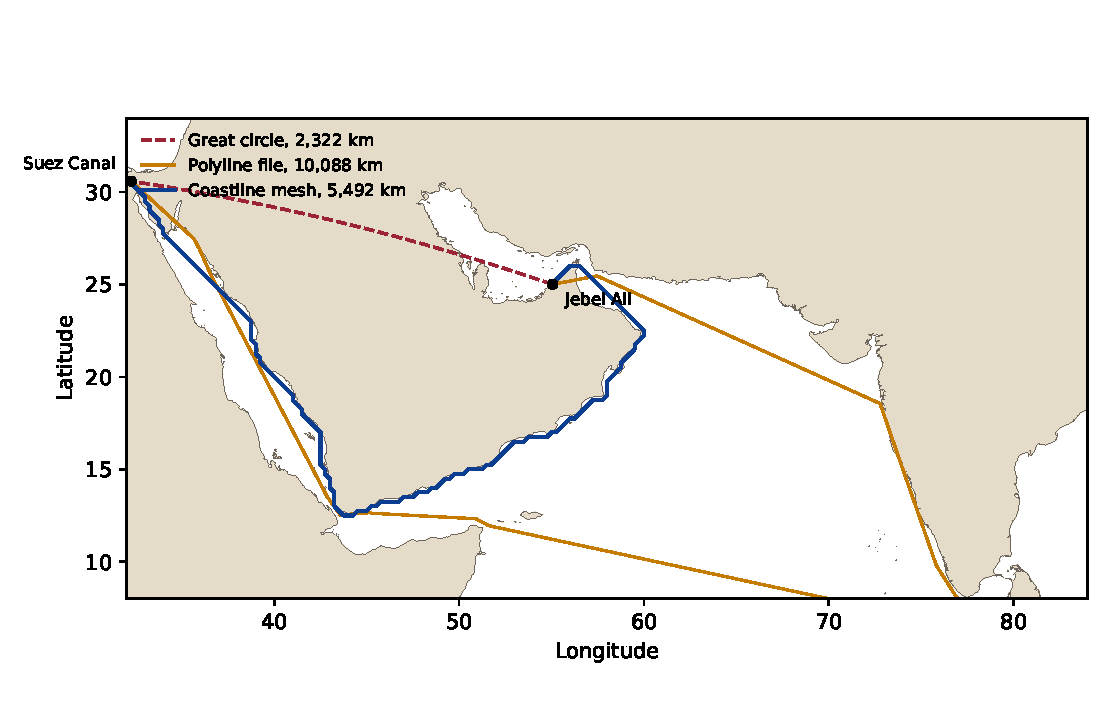
\includegraphics[width=\textwidth]{figures/jebel_ali_suez_mesh.pdf}
\caption{Jebel~Ali to the Suez Canal point used in the polyline study.
The dashed great circle crosses Arabia.
The coastline-mesh path enters the Bab el-Mandeb and does not go east of 62\(^\circ\)E.
The polyline-file path is drawn only because its length matches the stored 10{,}088~km figure.
It has \PolylineVertices{} vertices and a longest edge of \PolylineLongestEdgeKm~km.
Those edges are chords, not a coastline.
The file is not a navigable-water product.}
\label{fig:paths}
\end{figure}

% Generated by research/run_decomposition.py. Do not edit.
\begin{table}[t]
\centering
\caption{Distance and calm-water fuel at 18 knots. B1 is the great circle. It is not a feasible voyage when that arc crosses land. The deadline column is $F_2-F_{3,\mathrm{deadline}}$. B4 is omitted because no hindcast was cached.}
\label{tab:decomp}
\small
\begin{tabular}{lrrrrrr}
\toprule
Voyage & GC (km) & Mesh (km) & Ratio & $F_1$ (t) & $F_2$ (t) & Deadline (t) \\
\midrule
Jebel Ali--canal point & 2322 & 5492 & 2.366 & 165 & 390 & 0.0 \\
Jebel Ali--Suez port & 2284 & 5428 & 2.377 & 162 & 385 & 0.0 \\
New York--Rotterdam & 5858 & 6405 & 1.093 & 416 & 455 & 0.0 \\
\bottomrule
\end{tabular}
\end{table}


On the endpoints of the earlier polyline calculation, Jebel~Ali to 30.585\(^\circ\)N, 32.265\(^\circ\)E, the great circle is 2{,}322~km and crosses Arabia.
The mesh path is 5{,}492~km, ratio 2.37, and it enters the Bab el-Mandeb.
The polyline file's shortest stored path on those endpoints was 10{,}088~km, ratio 4.35.
It has \PolylineVertices{} vertices.
\PolylineLongEdges{} edges are longer than 1{,}000~km, and the path reached about 80\(^\circ\)E before turning west.
The longest edge is \PolylineLongestEdgeKm~km.
Figure~\ref{fig:paths} draws those edges as straight chords.
That is the file, not a sea track.
Of that file's excess over the great circle, the coastline mesh removes the eastward detour and leaves the continent.
The remaining factor of 2.37 is the feasible sea passage out of the Persian Gulf, across the Arabian Sea, and up the Red Sea.
It is not a routing improvement over the great circle, because the great circle is not a route.

At 18~knots the calm-water fuel is proportional to distance.
The same pair uses 165~t on the great circle and 390~t on the mesh.
The network term is \(+225\)~t.
A saving reported against the great circle on this corridor would be a negative number attached to an infeasible baseline.

New York--Rotterdam is the contrasting case.
The ratio is 1.09.
The great circle is nearly a sea path, and the mesh adds the remainder.
A 23--59\% Atlantic saving of the kind reported by \citet{bers2026} cannot be attributed to this network term.
Whatever that study is measuring, it is not the land mask we apply here.
We do not recompute their experiment.

The deadline-constrained speed term is 0.0~t on both voyages.
Under calm water the fuel-minimizing constant speed that meets the 18-knot arrival is 18~knots.
A speed saving against that arrival requires either a slower schedule, which is a different voyage, or a resistance that varies along the path, which is weather.
The commercial minimum at the pre-registered prices of 600~USD/t and 25{,}000~USD/day is 13~knots on the Jebel~Ali mesh path.
It uses less fuel because it takes longer.
It is not the 7\% speed lever in the SINTEF exercise, which holds the arrival time and changes the throttle against weather \citep{sintef2026ecorouter}.

No \(F_4\) is reported.
The kill rule in the pre-registration file forbids a weather percentage when the cache is empty.
Automatic Identification System tracks were not obtained.
Free feeds do not cover these crossings, and constructing tracks would have produced a model-versus-model comparison presented as if it were a voyage.
That was not done.

\section{What this does not show}

It does not show a weather-routing benefit, a genetic-algorithm benefit, or a calibrated fuel model.
The genetic algorithm in the accompanying application is a waypoint sequencer on a polyline graph.
It is not used here.
It does not show that \citet{mohamed2025} are wrong on Europe--Asia corridors; they used a different mask, a different resolution, and forced waypoints rather than cells.
It does not show that \citet{bers2026} overstated an Atlantic saving by ignoring land.
On our Atlantic pair the land correction is 9\%, not tens of percent.
It does not show an operational route for a ship.
The strait cells are opened by hand, depth is ignored, and the resistance model has not been compared with a noon report.

\section{Conclusion}

On these two corridors the identifiable gap between a great circle and a coastline-masked sea path is a property of the geography, not of an optimizer.
Where the arc crosses a continent the feasible path is 2.37 times as long, and an undocumented lane file made the same pair 4.35 times as long by missing the Gulf of Aden.
Where the arc is already at sea the factor is 1.09.
A fixed arrival in calm water adds no further fuel term.
A weather term, and a comparison with real tracks, are the remaining measurements.
Until they are in the cache, a percentage against the great circle is not a saving.

\paragraph{Data and code.}
Natural Earth 10~m land is stored under \texttt{data/raw}.
\texttt{research/run\_decomposition.py} writes \texttt{paper/decomposition\_results.json} and \texttt{paper/decomp\_table.tex}.
\texttt{paper/metrics\_preregistered.json} is the formula file and is not rewritten by that script.
\texttt{Shipping\_Lanes\_v1.geojson} is not a navigable-water product and is not an Automatic Identification System product.
No licence to redistribute Automatic Identification System tracks is claimed, because no such tracks are in the repository.

\bibliographystyle{plainnat}
\bibliography{references}

\end{document}
